% Slides accompanying "Learn RISC-V CPU Implementation and BSV" book
% Copyright (c) 2024 Rishiyur S. Nikhil, All Rights Reserved

% -*- mode: fundamental -*-

% Slides accompanying "Learn RISC-V CPU Implementation and BSV" book
% Copyright (c) 2024 Rishiyur S. Nikhil, All Rights Reserved

% This is a preamble shared by all the slide decks

\documentclass[10pt, aspectratio=169]{beamer}

% \documentclass[17pt]{beamer}

% Avail. font sizes: 8pt, 9pt, 10pt, 11pt, 12pt, 14pt, 17pt, 20pt.
% Default font size is 11pt (= 22pt in full screen mode).

\usepackage{verbatim}
\usepackage{fancyvrb}
\usepackage{listings}

% ================================================================
% Themes

\usetheme{Madrid}          % Line at bottom: Author (affiliation), OptTitle, Conf, page 

% \usetheme{Copenhagen}    % Same as Madrid except bottom line: Author, OptTitle

% \usetheme{Berkeley}    % Takes up 1-inch border on left and top

% ----------------
% colorthemes
% (default), beaver, beetle, seahorse, wolverine

\usecolortheme{seahorse}

% ================================================================
% Customization: show table of contents before each section
% Use \AtBeginSubsection    to show before each subsection

% \AtBeginSection[]
% {
%   \begin{frame}
%     \frametitle{Table of Contents}
%     \tableofcontents[currentsection]
%   \end{frame}
% }

% ================================================================

% ----------------
% The bsc compiler and BSV language
\newcommand{\bsc}{\emph{bsc}}
\newcommand{\BSV}{\bf{BSV}}
% ----------------
% ITALICISE WORDS
\newcommand{\ie}{\emph{i.e.,}}
\newcommand{\eg}{\emph{e.g.,}}
\newcommand{\Eg}{\emph{E.g.,}}
\newcommand{\etc}{\emph{etc.}}
\newcommand{\via}{\emph{via}}
\newcommand{\vs}{\emph{vs.}}

% ----------------
% EMPTY BOXES OF VARIOUS WIDTHS, FOR INDENTATION

\newcommand{\hm}{\hspace*{1em}}
\newcommand{\hmm}{\hspace*{2em}}
\newcommand{\hmmm}{\hspace*{3em}}
\newcommand{\hmmmm}{\hspace*{4em}}

% ----------------
% Convenient widths

\newlength{\hlessmm}
\setlength{\hlessmm}{\textwidth}
\addtolength{\hlessmm}{-2em}

\newlength{\hlessmmm}
\setlength{\hlessmmm}{\textwidth}
\addtolength{\hlessmmm}{-3em}

\newlength{\hlessmmmm}
\setlength{\hlessmmmm}{\textwidth}
\addtolength{\hlessmmmm}{-4em}

% ================================================================
% Title page

\title[Learn CPU design \& BSV]{Learn RISC-V CPU Implementation and BSV}

\subtitle{(BSV: a High-Level Hardware Design Language)}

\author[{\copyright} R.S.Nikhil]{Rishiyur S.~Nikhil}
% \institute{Bluespec, Inc.}

% Date is set differently in each slide deck

% \logo{
\includegraphics[height=0.6cm]{../Figures/Bluespec_Logo_2022-10}}

% End of preamble
% ****************************************************************


\date{L9: {\BSV}: Finite State Machines/StmtFSM}

% ****************************************************************

\begin{document}

% ================================================================

\begin{frame}
 \titlepage

 \begin{center}
  
\includegraphics[height=1cm]{Bluespec_Logo_2022-10}
 \end{center}

\end{frame}

% ================================================================

% -*- mode: fundamental -*-

% ================================================================

\begin{frame}[fragile]
\frametitle{Reminders}

\footnotesize

Please git clone: \url{https://github.com/rsnikhil/Learn_Bluespec_and_RISCV_Design} \\
(git pull for latest version).  Repsitory structure:

\vspace{1ex}

\begin{minipage}{0.5\textwidth}\scriptsize
\begin{Verbatim}[frame=single, numbers=left]
    ./Book_BLang_RISCV.pdf
      Slides/
          Slides_01_Intro.pdf
          Slides_02_ISA.pdf
          ...
      Exercises/
          Ex-03-A-Hello-World/
          Ex-03-B-Top-and-DUT/
          ...
      Code/
          src_Top/
          src_Drum/
          src_Fife/
          src_Common/
          ...
      Doc/Installing_bsc_Verilator_etc.{adoc,html}
\end{Verbatim}
\end{minipage}
\hm
\begin{minipage}{0.45\textwidth}
\begin{itemize}

 \item Slides and Exercise are numbered in sync with book Chapter numbers.

 \item For Exercises, please see Appendix E of the book.  Some (not
       all) exercises have associated code in the {\tt Exercises/}
       directory.

\end{itemize}
\end{minipage}

\vspace{2ex}

To compile and run the code for exercises, Drum and Fife, please make sure you have installed:

\begin{itemize}

 \item \emph{bsc} compiler (see \url{https://github.com/B-Lang-org/bsc})

 \item Verilator compiler (see \url{https://www.verilator.org/})
\end{itemize}

\footnotesize

\end{frame}

% ================================================================

\begin{frame}
\frametitle{Chapter Roadmap}

\footnotesize

\begin{center}
\frame{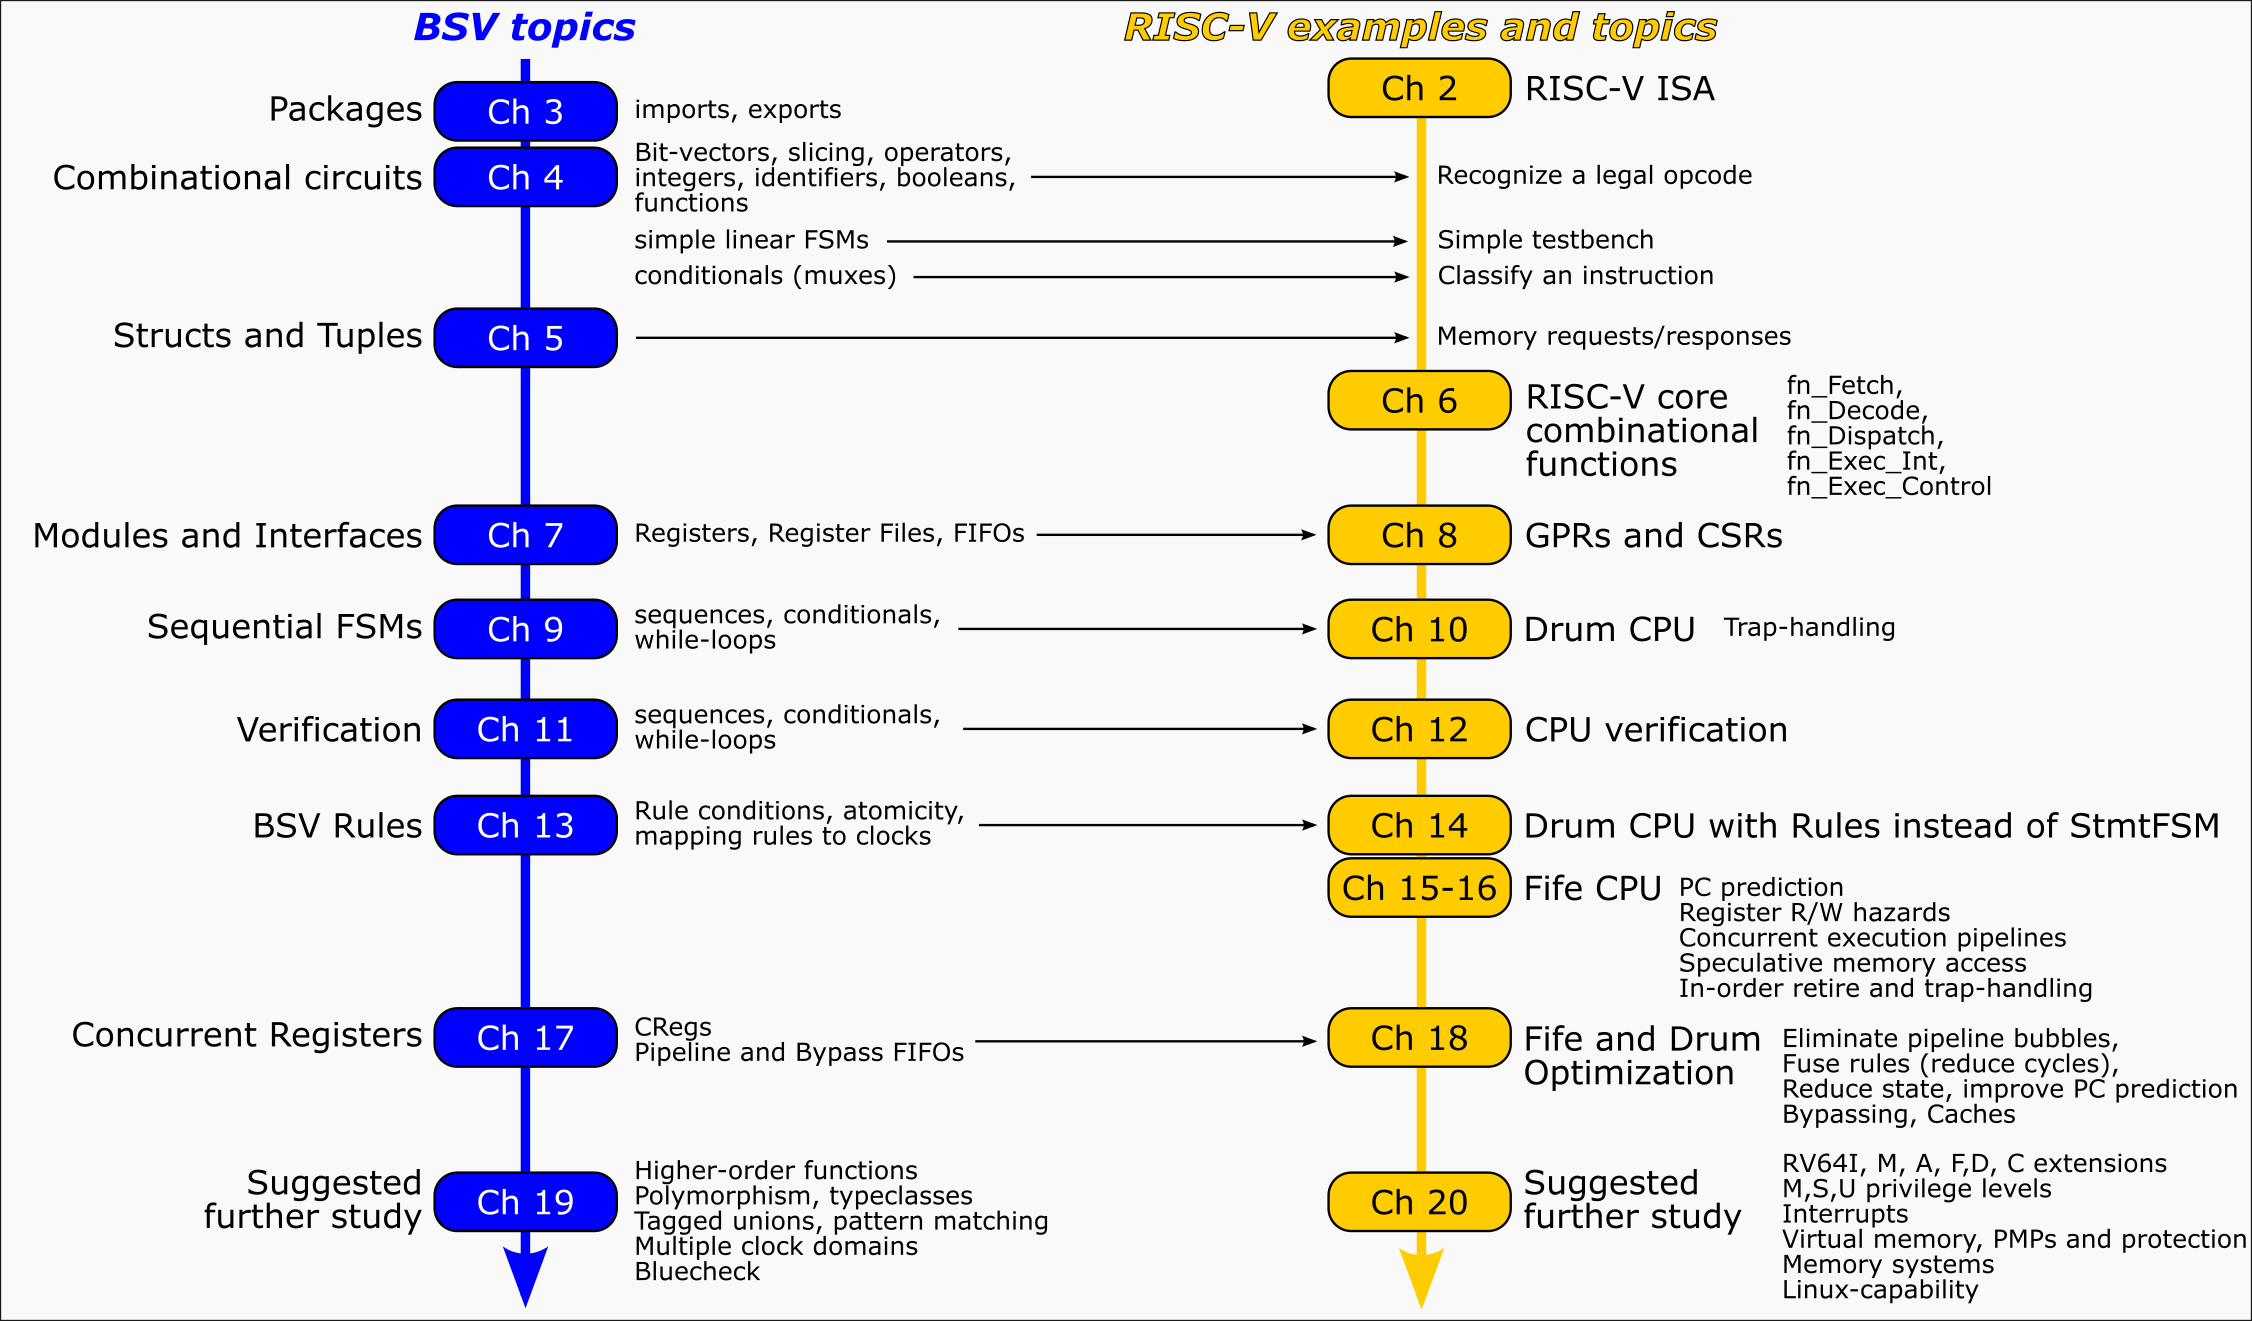
\includegraphics[height=0.825\textheight]{Fig_Chapter_Roadmap}}
\end{center}

\end{frame}

% ================================================================


% ================================================================

\begin{frame}
\frametitle{Flow of information between stages in Drum and Fife}

\footnotesize

\begin{center}
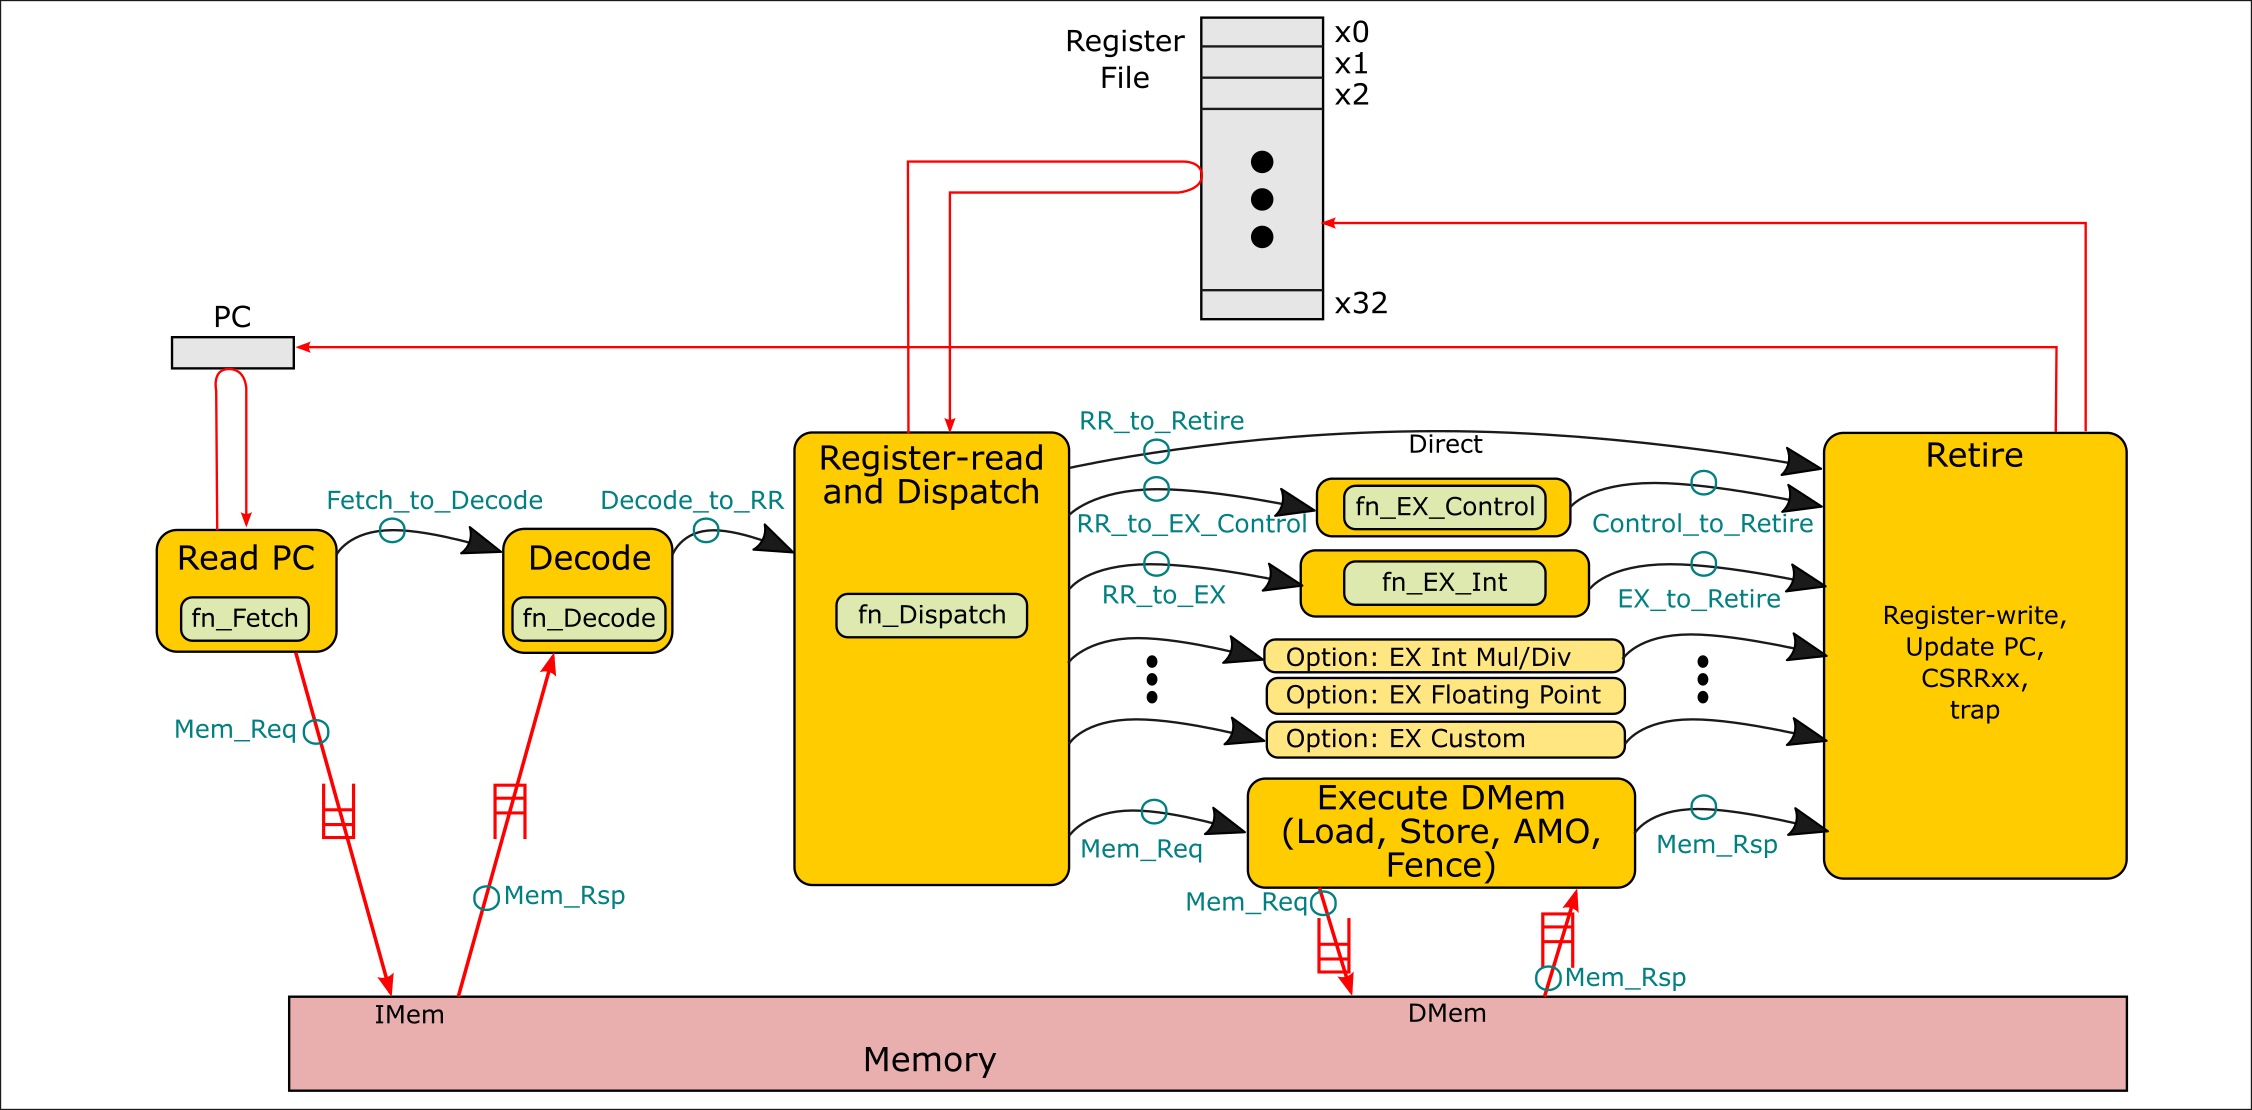
\includegraphics[height=0.6\textheight]{Fig_Instr_Exec_w_structs}
\end{center}

\end{frame}

% ================================================================

\begin{frame}[fragile]
\frametitle{Classical Finite State Machines (FSMs): Bubble-and-Arrow diagrams}

\footnotesize

An FSM is a \emph{process}, a behavior that evolves over time.

\vspace{1ex}

A classical notation for describing/specifying FSMs is the bubble-and-arrow diagram.

\vspace{1ex}

Here is a (greatly over-simplified) FSM spec for controlling an elevator:

\begin{center}
\includegraphics[width=\textwidth]{Fig_FSM_Bubble_and_Arrow}
\end{center}

Each state of the process is depicted by a bubble.  Each arrow depicts
a transition to another state enabled by a condition ({\bf C:}) and
performing an action ({\bf A:}).

\PAUSE{\vspace{5ex}}

The RISC-V instruction-execution flow diagram can be interpreted as an
FSM bubble-and-arrow diagram, and implemented that way.  This is
exactlly what Drum is.

\end{frame}

% ================================================================

\begin{frame}[fragile]
\frametitle{Sequential {\vs} Concurrent FSMs}

\footnotesize

Most hardware systems (except for extremely simple ones) are best viewed as \emph{communicating, concurrent FSMs}:

\begin{center}
\includegraphics[width=\textwidth]{Fig_FSMs_Concurrent}
\end{center}

Multiple FSMs communicate with each other ({\via} registers, register files, FIFOs, ...).

\PAUSE{\vspace{5ex}}

\emph{Note:} theoretically multiple FSMS are equivalent to a single FSM, but
the size of such a single-FSM description can be MUCH larger.  This is
because we have to describe all possible combinations of states where
when one FSM is in state $A_j$ and and another FSM is simultaneously
in state $B_k$.

\end{frame}

% ================================================================

\begin{frame}[fragile]
\frametitle{{\BSV}: {\tt StmtFSM}: sub-language for specifying structured FSMs}

\footnotesize

{\tt StmtFSM} is a sub-language in {\BSV} for specifying structured FSMs.
\begin{itemize}

 \item We start with an expression of type {\tt Action}.

 \item Then, we \emph{compose} larger FSMs from smaller FSMs using
       sequencing, if-then-else and while-loop constructs.

\end{itemize}

\vspace{2ex}

\begin{center}
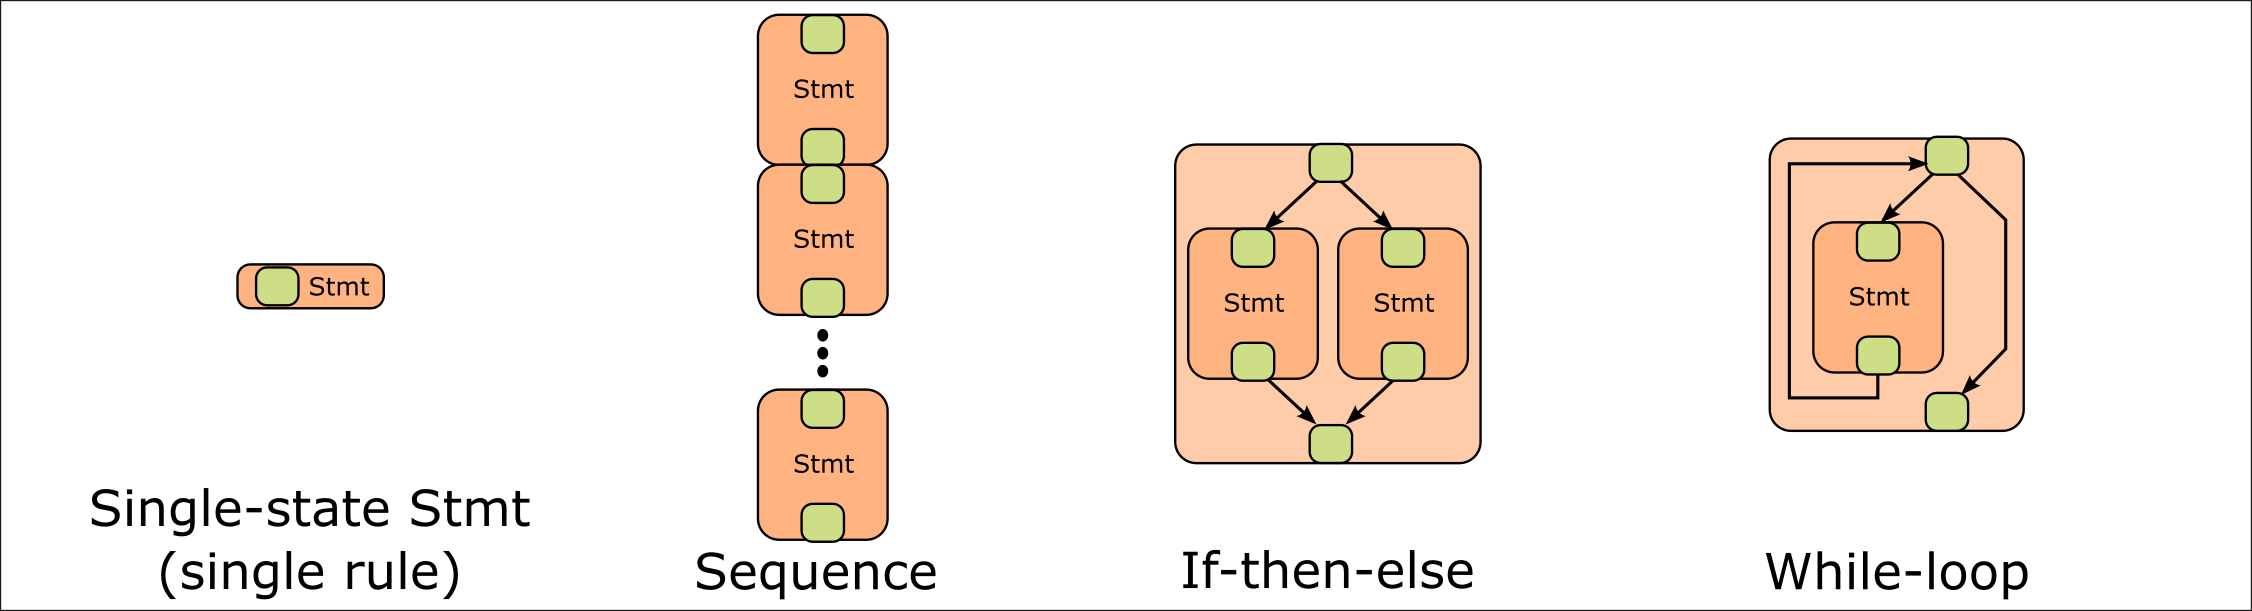
\includegraphics[width=\textwidth]{Fig_FSMs_Structured}
\end{center}

\vspace{2ex}

Each construct produces an expression of type {\tt Stmt}.

\end{frame}

% ================================================================

\begin{frame}[fragile]
\frametitle{{\BSV}: A single-state FSM}

\footnotesize

Example:

\vspace{2ex}

\begin{Verbatim}[frame=single]
   seq
      action
         rg_pc <= rg_pc + 4;          // Assignment to a register
         f_F_to_D.deq;                // Dequeue a fifo
         f_D_to_RR.enq (v);           // Enqueue into a fifo
         $display ("Hello, World!");  // Print something (in simulation only)
      endaction
   endseq
\end{Verbatim}

\vspace{2ex}

The {\tt seq}-{\tt endseq} construct is an expression of type {\tt Stmt}.

\vspace{4ex}

All actions in an {\tt action}-{\tt endaction} block take
place \emph{simultaneously} and \emph{instantaneously}, no matter the
textual order in which they are written.

\vspace{1ex}

(In hardware, all their ENABLE signals are asserted simultaneously,
and they are all performed on the next clock signal.)

\end{frame}

% ================================================================

\begin{frame}[fragile]
\frametitle{{\BSV}: Action-blocks can contain name-bindings}

\footnotesize

Example:
\begin{Verbatim}[frame=single, numbers=left]
   action
      Bit #(XLEN) next_pc = rg_pc + 4;
      rg_pc <= next_pc;
      $display ("Next PC is %08h", next_pc);
      ...
      let y <- pop_o (to_FIFOF_O (f_mem_rsps));
      ...
      $display ("mem_rsp is ", fshow (y));
   endaction
\end{Verbatim}

\end{frame}

% ================================================================

\begin{frame}[fragile]
\frametitle{{\BSV}: Linear Sequence flows}

\footnotesize

\begin{Verbatim}[frame=single]
   seq
      ... Action or Stmt ...
      ... Action or Stmt ...
      ...
      ... Action or Stmt ...
   endseq
\end{Verbatim}

\emph{Note:} A sequence of $n$ actions may not complete in $n$ clocks.  \\
Actions execute according to usual {\BSV} semantics---an action may
implicitly stall (be paused) until all the methods it invokes are
READY.

\PAUSE{\vspace{2ex}}

Library-provided actions to explicitly pause an FSM:
\begin{Verbatim}[frame=single]
   seq
      ...
      await (... Bool expr ...)        // pause until some condition
      delay (... numeric expr ...)     // pause for n cycles
      ...
   endseq
\end{Verbatim}

\end{frame}

% ================================================================

\begin{frame}[fragile]
\frametitle{{\BSV}: Conditional and loop flows}

\footnotesize

Conditional flows:
\begin{Verbatim}[frame=single]
   if (... Bool expr ...)
      ... Action or Stmt ...
   else
      ... Action or Stmt ...
\end{Verbatim}

\vspace{2ex}

Note: ``if (b) ... else ...'' is used in {\BSV} in two different ways:

\begin{itemize}
 \item In computation, where they represent hardware MUXes (multilexers)
 \item In {\tt StmtFSM}, where they represent alternative temporal FSM flows
\end{itemize}

But there is no ambiguity, because these are distinct contexts.

\PAUSE{\vspace{5ex}}

Loop flows:
\begin{Verbatim}[frame=single]
   while (... Bool expr ...)
      ... Action or Stmt ...
\end{Verbatim}

\end{frame}

% ================================================================

\begin{frame}[fragile]
\frametitle{{\BSV}: Instantiating an FSM from a {\tt Stmt} specification}

\footnotesize

\begin{Verbatim}[frame=single, numbers=left]
   mkAutoFSM (... argument expression of type Stmt ...);
\end{Verbatim}

\begin{itemize}
        
 \item This statement occurs inside a module, along with other sub-module instantiations.

 \item This statement instantiates a sub-module whose behaviour is specified by the {\tt Stmt}

 \item The FSM starts running as soon as the system comes out of reset.

 \item If the FSM reaches its end state, it executes a {\tt \$finish()} to stop simulation.

       Note:
       \begin{itemize}
        \item (It may not reach the end state if it has an infinite while-loop.)

        \item (It may not reach the end state if some action gets stuck,
              {\eg} trying to dequeue an empty FIFO.)
       \end{itemize}
\end{itemize}

\end{frame}

% ================================================================

\begin{frame}[fragile]
\frametitle{{\BSV}: {\tt StmtFSM} final comments}

\footnotesize

\begin{itemize}
        
 \item {\tt StmtFSM} is frequently used in testbenches for
        sequentially producing test stimulus and squentially consuming
        outputs (although, in Drum, we also use it in the design).

 \item {\tt StmtFSM} can only express \emph{structured} processes.
       For more complex flows, we directly use {\BSV} \emph{Rules}
       ({\eg} in Fife).

\end{itemize}

\PAUSE{\vspace{5ex}}

\begin{itemize}
        
 \item There are more ways to create {\tt Stmt}'s; see {\bsc} library document.

 \item There are more module-constructors (than {\tt mkAutoFSM}); see {\bsc} library document.

\end{itemize}

\end{frame}

% ****************************************************************

% -*- mode: fundamental -*-

% Slides accompanying "Learn RISC-V CPU Implementation and BSV" book
% Copyright (c) 2024 Rishiyur S. Nikhil, All Rights Reserved

% This is a postamble shared by all the slide decks

% ================================================================

\begin{frame}

\begin{center}
  {\LARGE End}
\end{center}

\end{frame}

% ================================================================


% ****************************************************************

\end{document}
% ****************************************************************
